\chapter{Results}
This chapter should encompass your data analysis and findings. Additionally, include relevant tables, figures, and citations to support your results and interpretations. Here is a suggested list of topics to discuss:
\section{Interface Comparison}
During the development of this project, various experiments were conducted to optimize the performance of a quantum molecular simulator. In this context, the choice of the interface for calculating cost functions is crucial, as these functions must be optimized to obtain the optimal state and geometry of each molecule. Typically, the \textit{JAX} interface is the most widely used due to its GPU acceleration capabilities, which generally provide greater efficiency and speed in searching for the minimum of the cost function.

However, when comparing two identical implementations—varying only the calculation interface—we observed an unexpected result: the \textit{JAX}-based interfacerunning on a GPU was slower than the \textit{autograd}-based interface on a CPU. To confirm that this was not a coding error, we repeated the experiments on different machines, obtaining the same result. For this reason, we opted to continue with the \textit{autograd} interface due to its greater speed in our specific implementation.

\subsection{Optimization and Timing Logging}
To verify the performance differences between both interfaces, the same optimization was executed while varying only the interface. During these simulations, the execution times of the different functions in the code were recorded, with their values shown in Table~\ref{tab:comparison_gd}.

\begin{table}[H]
  \centering
  \scriptsize
  \resizebox{\textwidth}{!}{%
  \begin{tabular}{lcccccc}
  \toprule
  \textbf{Function} & 
  \textbf{[\texttt{Li}, \texttt{H}] \_autograd\_GD} & 
  \textbf{[\texttt{Li}, \texttt{H}] \_jax\_GD} & 
  \textbf{[\texttt{O}, \texttt{H}, \texttt{H}] \_autograd\_GD} & 
  \textbf{[\texttt{O}, \texttt{H}, \texttt{H}] \_jax\_GD} & 
  \textbf{[\texttt{H}, \texttt{H}] \_autograd\_GD} & 
  \textbf{[\texttt{H}, \texttt{H}] \_jax\_GD} \\
  \midrule
  Iteration 1  & 1246.7627 & 6251.3362 & 6942.21696 & 39003.89009 & 14.6908 & 40.5485 \\
  Iteration 2  & 1244.0321 & 6284.9812 & 6935.09353 & 40652.7751  & 14.7824 & 36.2979 \\
  Iteration 3  & 1247.4399 & 6348.2470 & 6920.68571 & 40386.29868 & 14.9931 & 38.6236 \\
  Iteration 4  & 1245.7256 & 6351.6437 & 6942.60873 & 40128.31419 & 15.0694 & 39.1362 \\
  Iteration 5  & 1244.8591 & 6349.5099 & 6965.70663 & 40657.74473 & 15.1512 & 40.6186 \\
  \midrule
  \textbf{Total Time} & 6228.8195 & 31585.7475 & 34706.3116 & 200829.0866 & 74.6870 & 195.2551 \\
  \textbf{build\_hamiltonian} & 29.1349   & 30.3407  & 78.4744   & 85.7532   & 0.4934   & 0.5329  \\
  \textbf{compute\_operator\_gradients} & 1533.0319 & 17497.4381 & 12563.3726 & 113792.7167 & 0.6313   & 11.9006 \\
  \textbf{update\_parameters\_and\_coordinates} & 4666.6385 & 14056.6795 & 22064.4153 & 86946.6021 & 73.5594 & 182.5271 \\
  \bottomrule
  \end{tabular}%
  }
  \caption{Execution times for different molecules and interfaces using \textit{Gradient Descent}.}
  \label{tab:comparison_gd}
\end{table}

Figure~\ref{fig:time_iterations} shows how the execution time evolves over the iterations for each molecule and type of interface. It is evident that, in all cases, the \textit{autograd}-based interface offers lower computation times than the \textit{JAX}-based interface.

\begin{figure}[H]
  \centering
  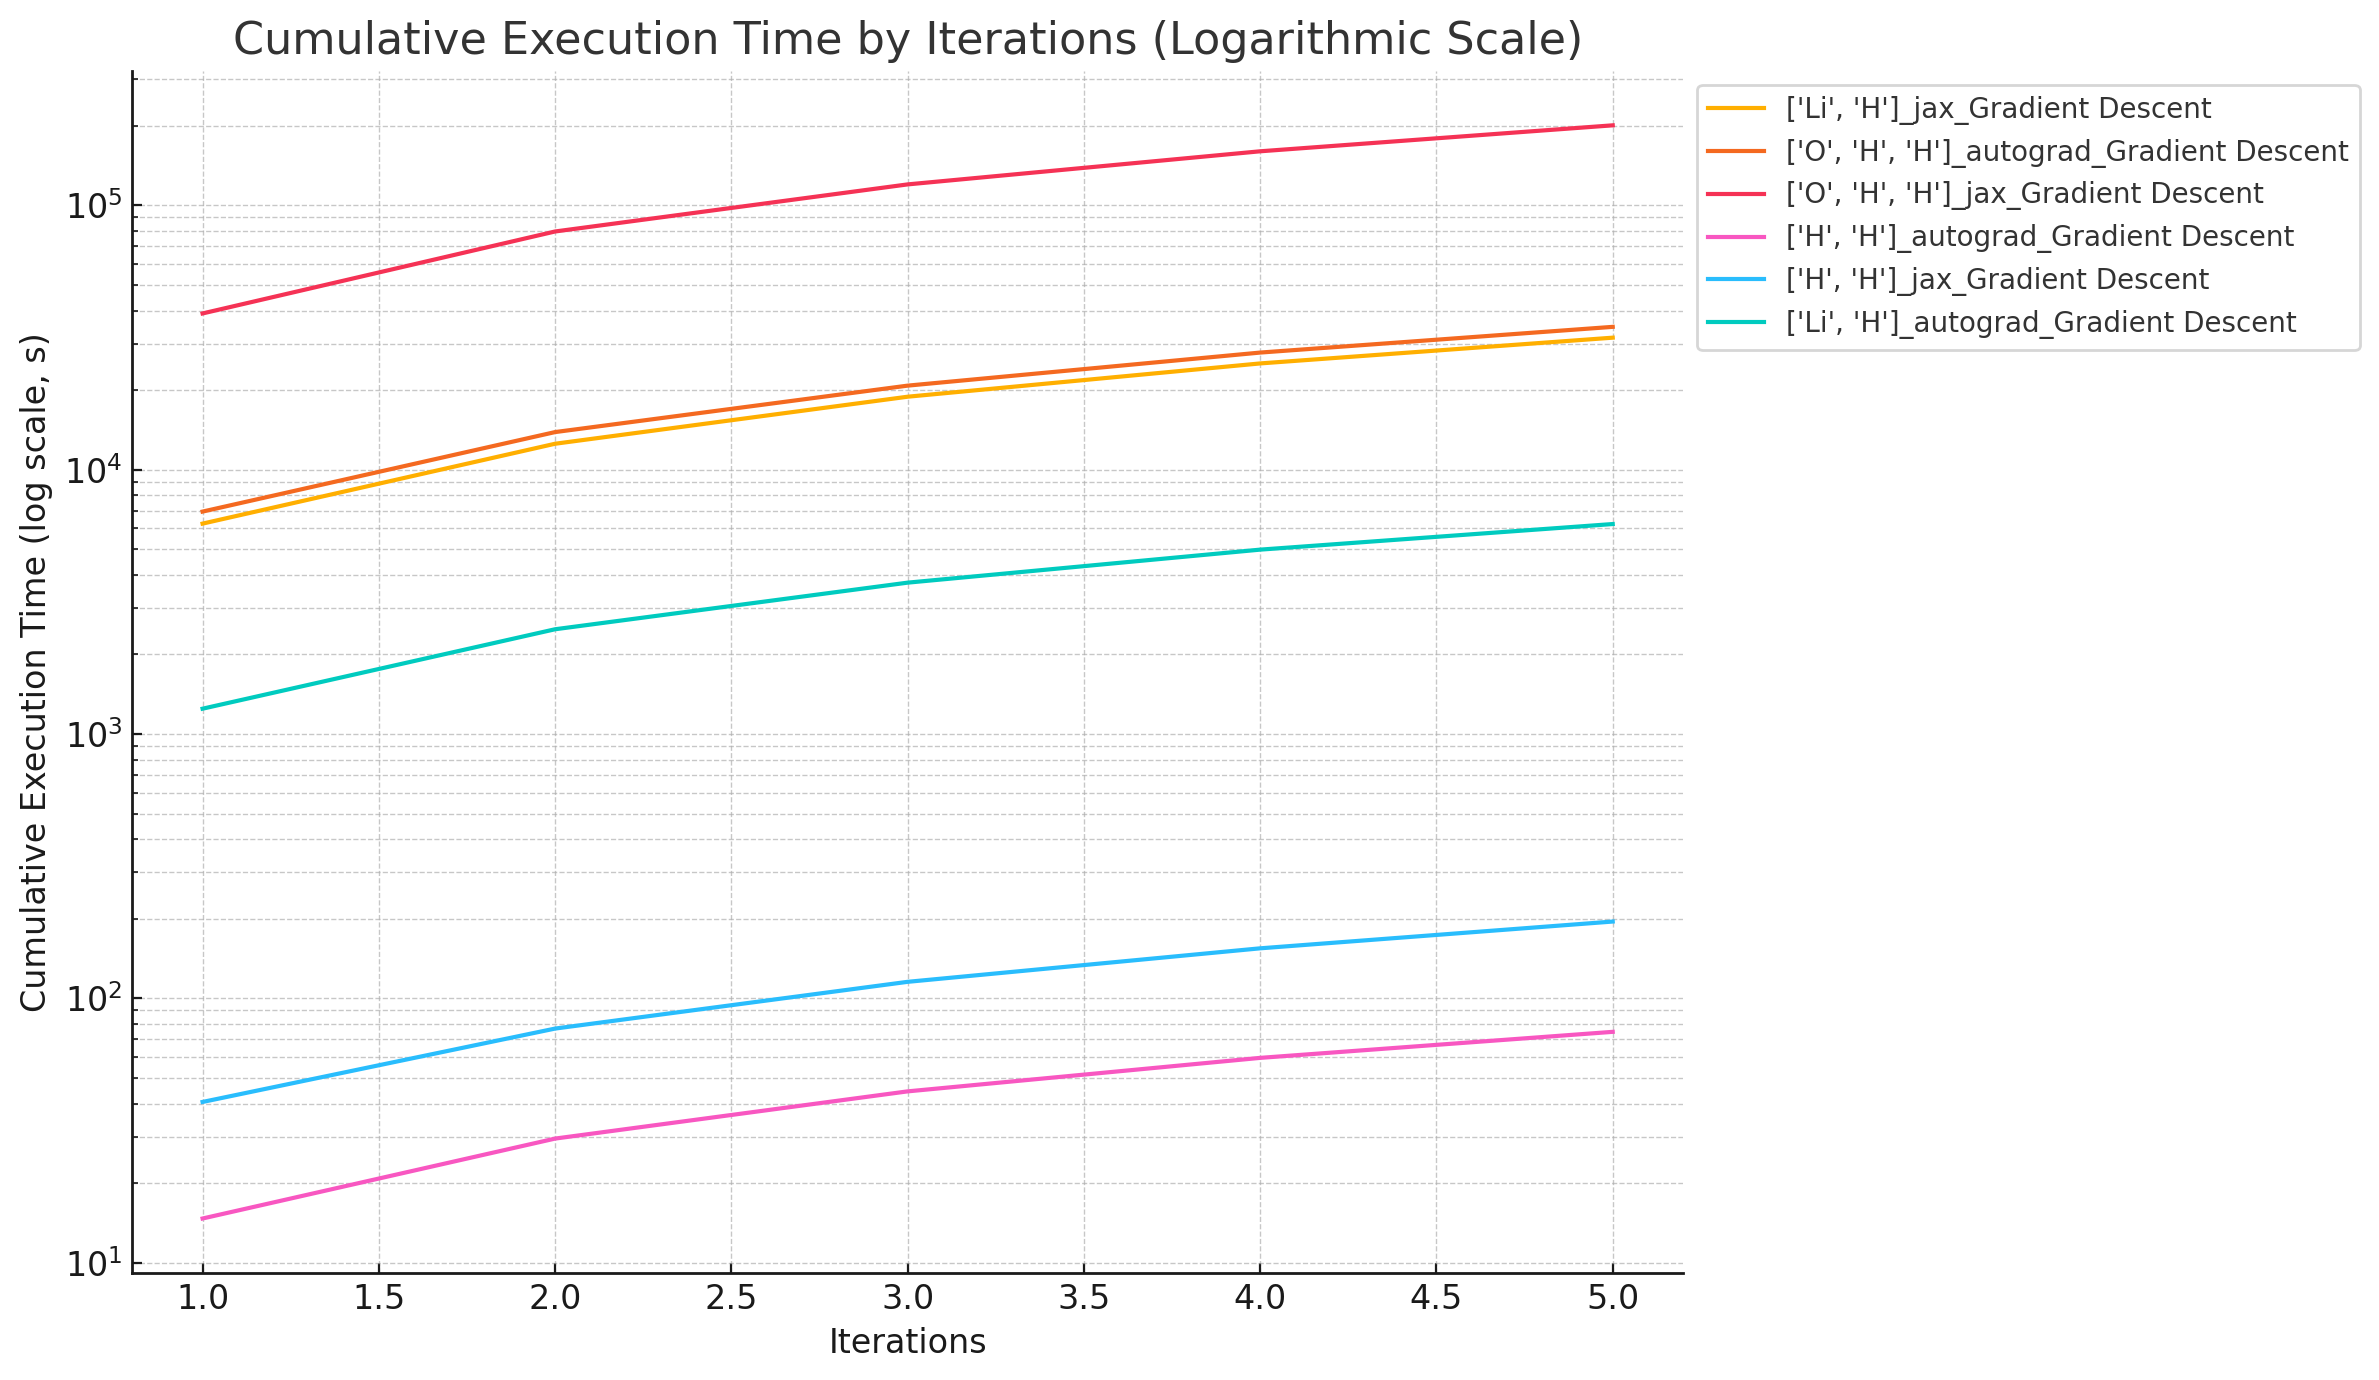
\includegraphics[width=0.8\textwidth]{img/time_iterations.png}
  \caption{Execution time of different molecules per iteration in the simulation.}
  \label{fig:time_iterations}
\end{figure}

\subsubsection{Comparative Performance Analysis}
To evaluate the performance of both interfaces in more detail, a table was created showing the percentage increase in execution time of \textit{JAX} compared to \textit{autograd}, as seen in Table~\ref{tab:jax_vs_auto}.

\begin{table}[H]
  \centering
  \scriptsize
  \resizebox{\textwidth}{!}{%
  \begin{tabular}{lcccc}
  \toprule
  \textbf{Metric} & 
  \textbf{LiH} & 
  \textbf{H\textsubscript{2}} & 
  \textbf{H\textsubscript{2}O} & 
  \textbf{Mean} \\
  \midrule
  \textbf{Total Time} & 80.28\% & 82.72\% & 61.75\% & 74.92\% \\
  \textbf{build\_hamiltonian} & 3.97\% & 8.49\% & 7.42\% & 6.63\% \\
  \textbf{compute\_operator\_gradients} & 91.24\% & 88.96\% & 94.70\% & 91.63\% \\
  \textbf{update\_parameters\_and\_coordinates} & 66.80\% & 74.62\% & 59.70\% & 67.04\% \\
  \bottomrule
  \end{tabular}%
  }
  \caption{Comparison of execution times between JAX and autograd interfaces for different molecules.}
  \label{tab:jax_vs_auto}
\end{table}

On average, it was observed that the \textit{JAX} interface exhibits a 74.92\% higher total execution time than the \textit{autograd} interface. Additionally, it is interesting to note that as the complexity of the molecule increases (with a greater number of atoms), the penalty percentage of \textit{JAX} tends to decrease. This behavior suggests that, in larger-scale problems, GPU acceleration could become more competitive, although it does not manage to outperform \textit{autograd} in this implementation.

\subsection{Computation Time per Function}
For a higher level of detail, the computation time was also measured for each part of the code where the interface change is introduced. Figure~\ref{fig:time_functions} shows the accumulated execution times in the main stages of the algorithm.

\begin{figure}[H]
  \centering
  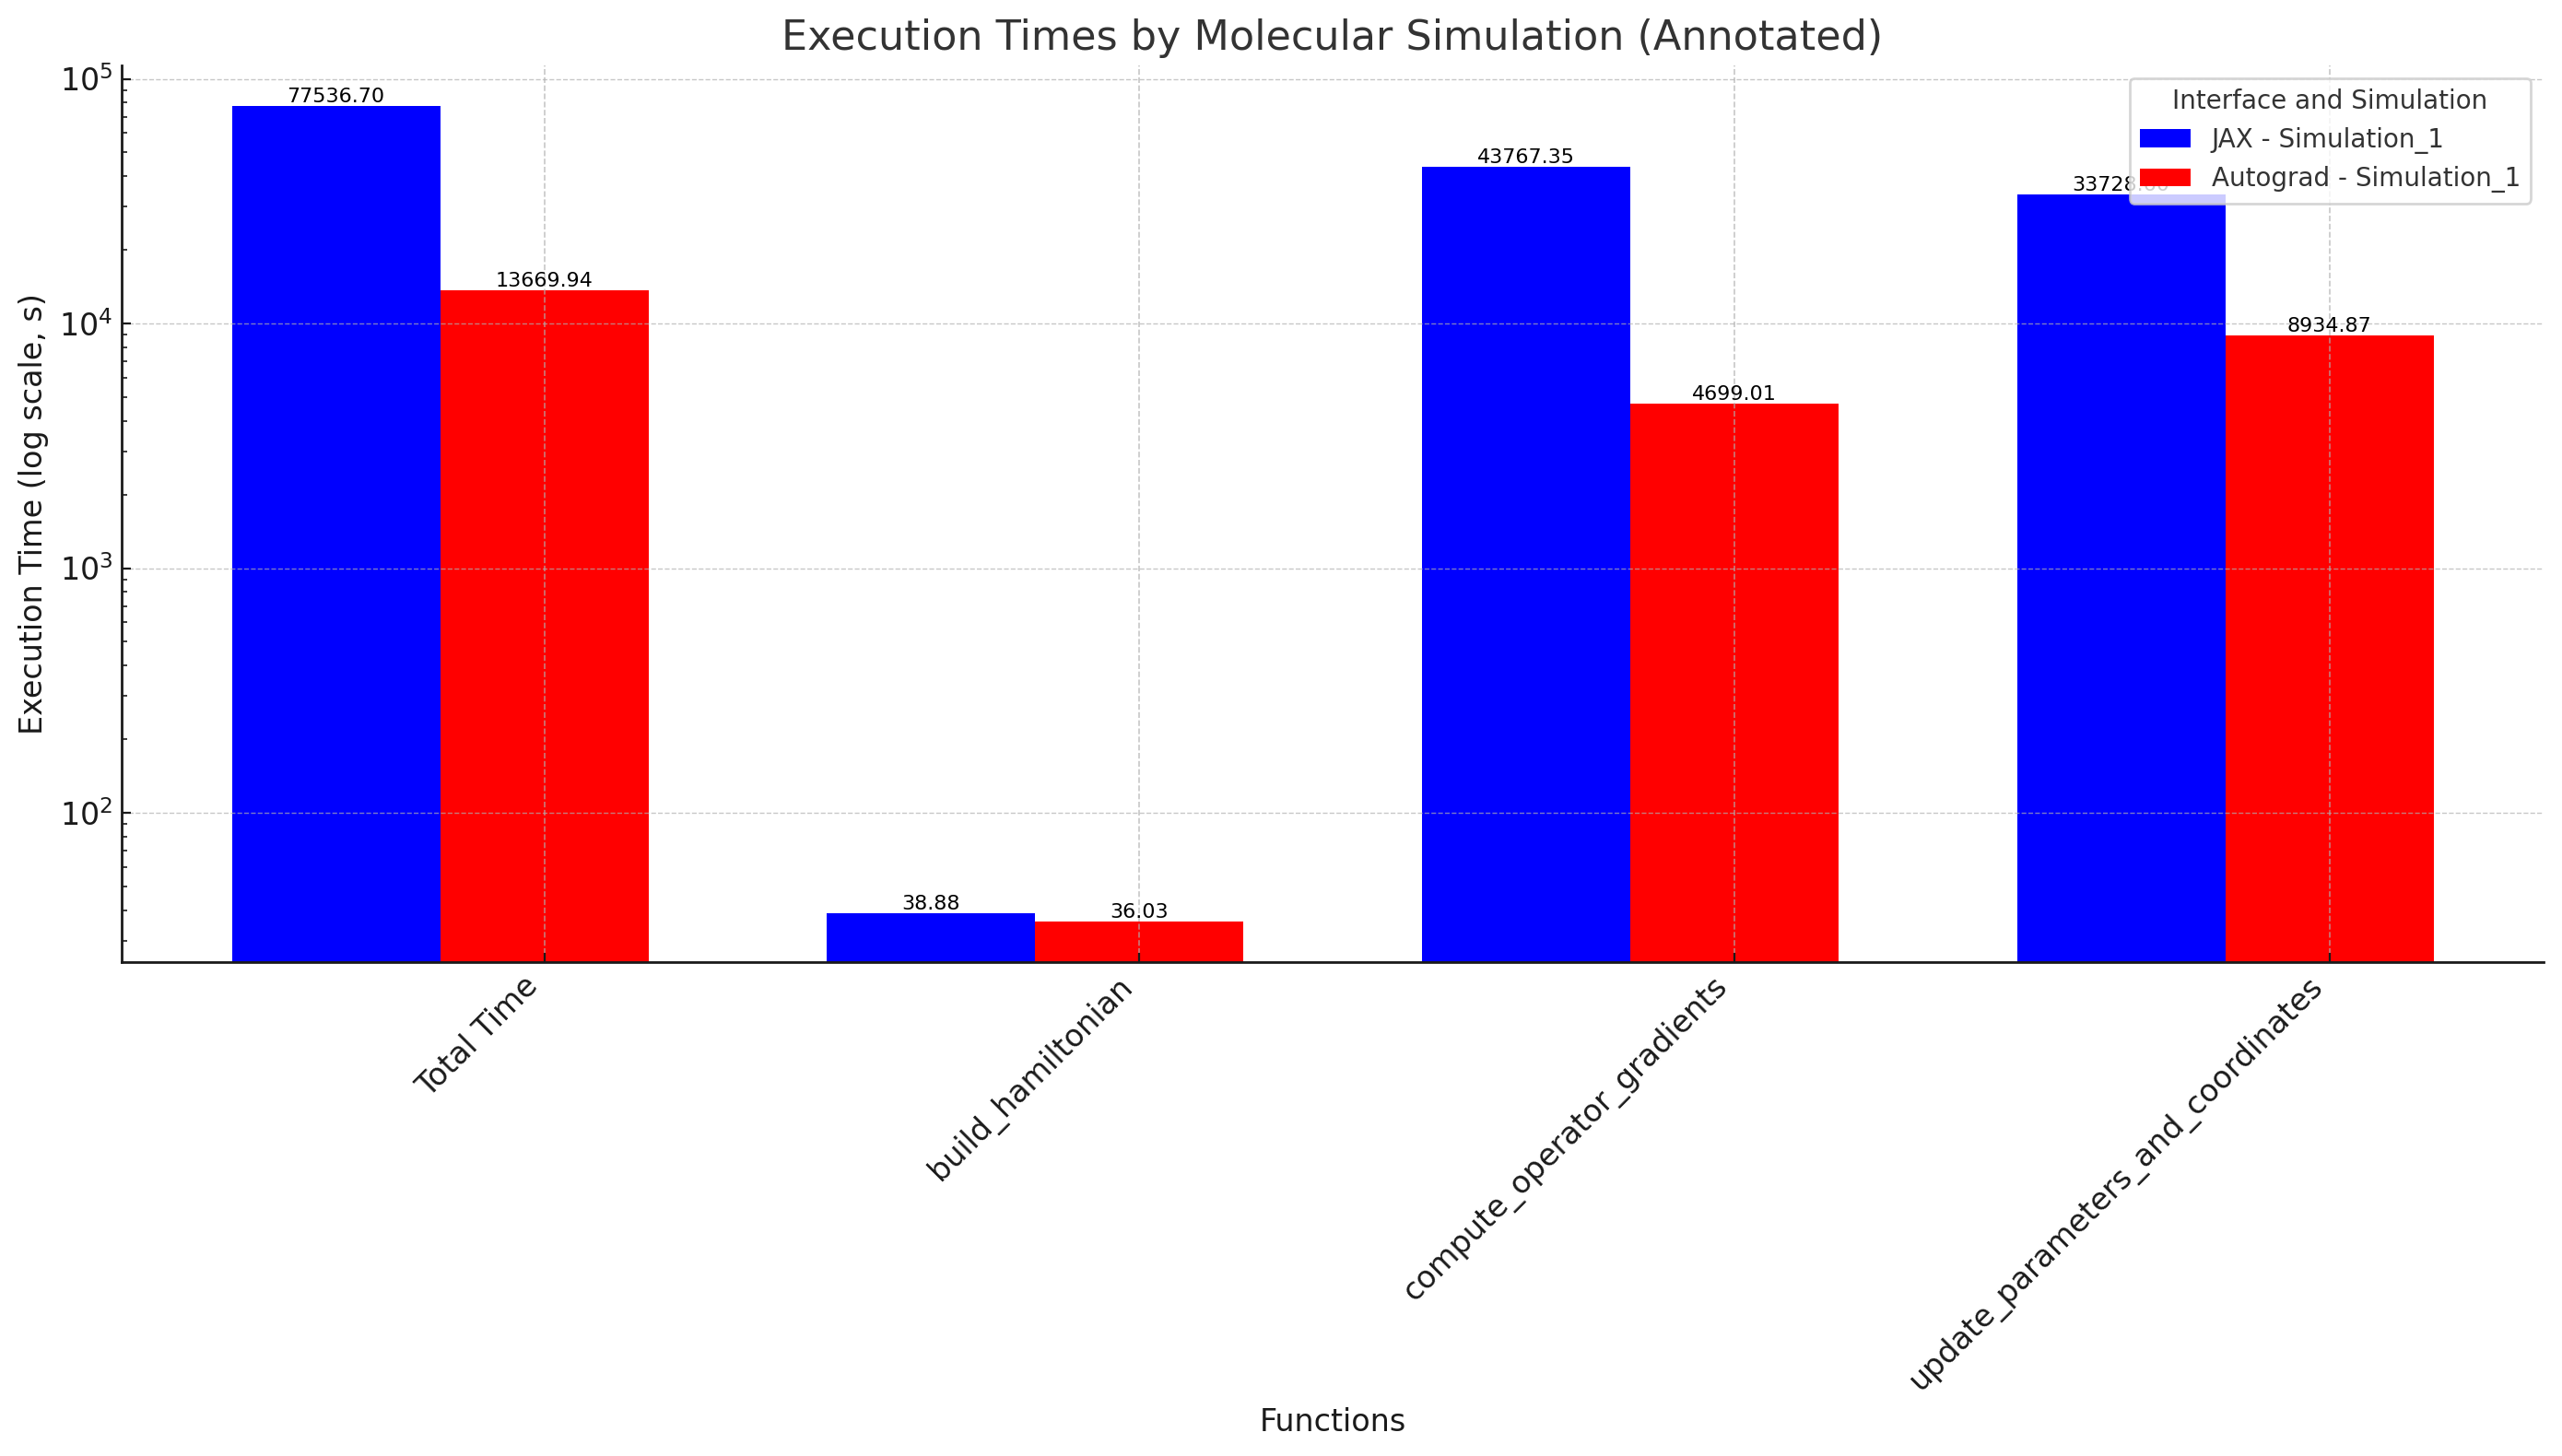
\includegraphics[width=0.8\textwidth]{img/time_functions.png}
  \caption{Execution time in different parts of the code.}
  \label{fig:time_functions}
\end{figure}

The same pattern is maintained in all functions: the \textit{JAX} interface records higher execution times than \textit{autograd}. In particular, the gradient computation part \texttt{compute\_operator\_gradients} increases its execution time by 91.68\% when using \textit{JAX}. This difference is largely attributed to the overhead caused by data transfer between the CPU and GPU, especially given that \textit{PennyLane} does not fully support Hamiltonian generation on the GPU.

On the other hand, the function \texttt{update\_parameters\_and\_coordinates}, responsible for performing the molecular geometry and parameter optimization step, also shows a 67.04\% increase when using \textit{JAX}. Nevertheless, it is worth highlighting that as the problem grows in complexity, the \textit{JAX} interface gains some relative efficiency in gradient calculation; however, the time saved through GPU acceleration is offset by the continuous data transfer between CPU and GPU throughout the iterations.

\subsection{Conclusions}
Based on the obtained results, the \textit{autograd} interface demonstrated superior performance in terms of speed for our implementation of the quantum molecular simulator. Although the GPU is usually advantageous in larger-scale problems, the data transfer overhead and the lack of full support for Hamiltonian generation within the GPU reduced the efficiency of \textit{JAX}. For this reason, we ultimately chose to use the \textit{autograd} interface for the final implementation of the quantum molecular simulator.

\section{Ansatz Comparison}
One of the most significant modifications affecting our code and its functionality has been the choice of the Ansatz. Our proposal has been to implement UCCSD, an Ansatz typically used for this type of simulation, as it enhances the simulation performance by achieving higher efficiency. The efficacy of this type of Ansatz has already been demonstrated, showing how it can improve simulation performance by producing more optimal quantum circuits without the need to create a specific Ansatz for the molecule being simulated. Indeed, for each optimizer configuration and for each different molecule simulation, there exists an optimal quantum circuit that achieves the best performance. However, since our objective is to develop a program that can simulate various molecules with maximum performance, we observe that the best option is UCCSD. To illustrate how our simulation performance is improved, we have generated Ansätze with different levels of depth and compared their performance with that of a UCCSD Ansatz. We have simulated various configurations of classical Ansätze, and in all cases, the UCCSD Ansatz has achieved better performance. More complex and molecule-specific Ansätze could be tested, but it is unlikely that another type of Ansatz would outperform UCCSD in terms of performance improvement.

Below is a simulation with different Ansatz depths and varying numbers of iterations obtained directly from the simulation.

\begin{figure}[H]
  \centering
  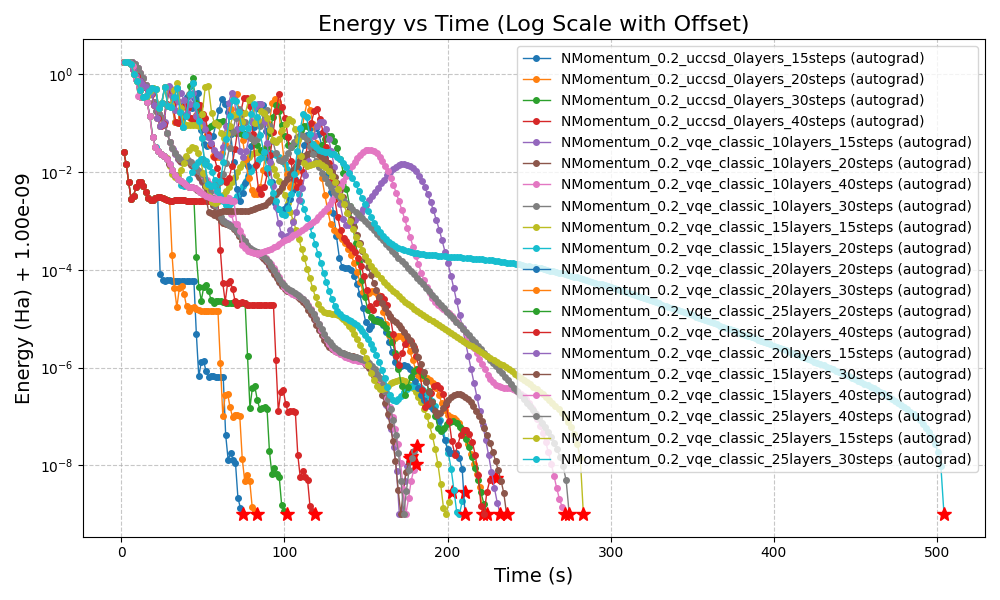
\includegraphics[width=0.8\textwidth]{data/Anzatz/results_ansatz_lyers_dif_iterations/energy_vs_time_log_offset.png}
  \caption{Energy vs. Time for different Ansätze and iterations.}
  \label{fig:ansatz_layers_iterations}
\end{figure}

It is observed that the UCCSD Ansatz achieves the best performance in all simulations, regardless of the number of optimizations performed for each iteration. For greater clarity of the results, a simulation was conducted with only a single number of optimizations per iteration, and the performance of the different Ansätze was compared, providing a clearer view of how UCCSD achieves the optimal performance.

\begin{figure}[H]
  \centering
  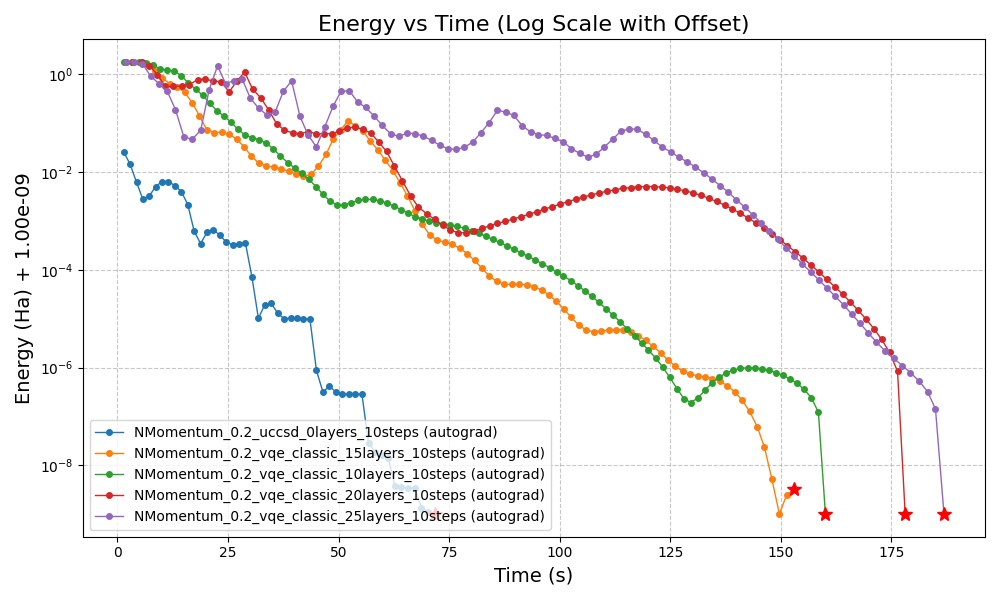
\includegraphics[width=0.8\textwidth]{data/Anzatz/results_ansatz_lyers/energy_vs_time_log_offset.png}
  \caption{Energy vs. Time for different Ansätze.}
  \label{fig:ansatz_layers}
\end{figure}

Finally, to corroborate that the UCCSD Ansatz achieves the best performance, a simulation was conducted with a different molecule, and the performance of the various Ansätze was compared. In the following image, it can be seen that the UCCSD Ansatz achieves highest efficiency in all simulations.

\section{Optimizer}

Once the Ansatz was selected, the next step was to test the functionality of our project, and thus see how it could help us improve the performance of our simulations. For this purpose, a series of tests were carried out using the capabilities previously designed for performance improvement. The tests were performed with a single Ansatz, UCCSD, and for the following molecules: H2, LiH, and H2O.

The steps followed for the realization of the tests were as follows:
\subsection{Optimizer Selection}
The first step was to determine the optimizer for the different molecules. To achieve this, we developed a procedure that allowed executing the same molecules with various optimizers, each covering a range of \emph{step size} values. This approach enabled the comparison of the different optimizers to be as fair as possible.

In the first phase, which executed 42 processes in parallel, observing which \emph{step size} offered the best performance for each optimizer and molecule. Subsequently, the simulation was repeated using only those optimal \emph{step sizes}, thereby achieving greater accuracy in the optimal \emph{step size} value for each optimizer, which will be discussed in the next section. The results of this second simulation are presented below.


\begin{figure}[H]
  \centering
  % First image
  \begin{subfigure}{0.45\textwidth}
    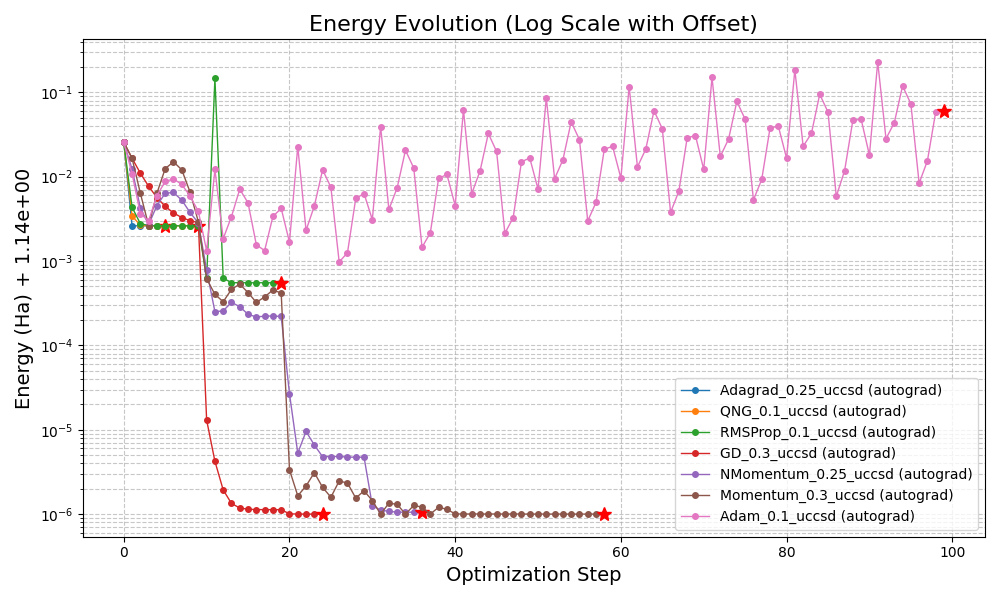
\includegraphics[width=\textwidth]{data/Optimizadores/final_results_H2/energy_evolution_log_offset.png}
    \caption{H2 simulation.}
    \label{fig:subimage1}
  \end{subfigure}
  % Second image
  \begin{subfigure}{0.45\textwidth}
    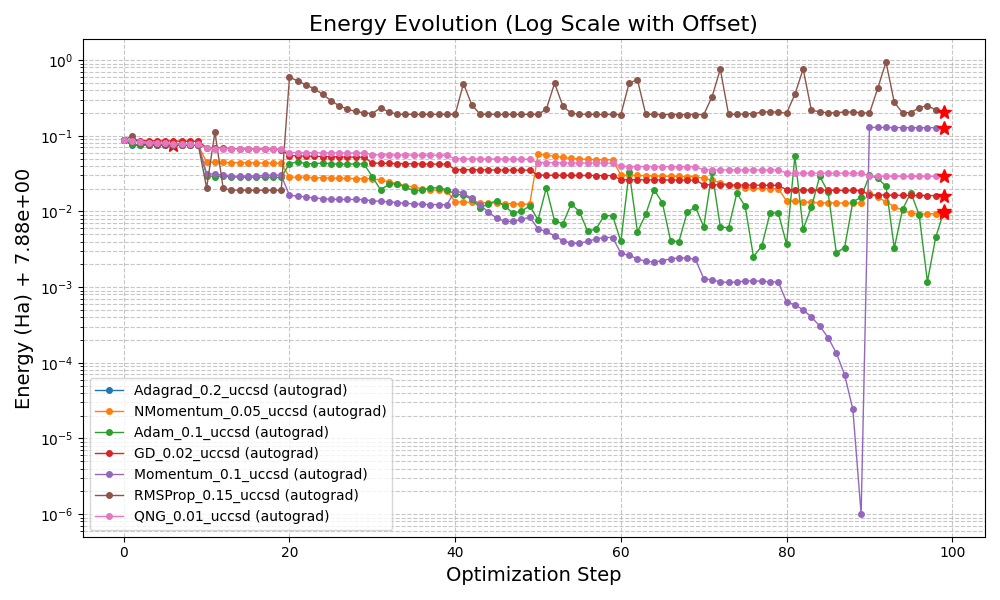
\includegraphics[width=\textwidth]{data/Optimizadores/final_results_LiH/energy_evolution_log_offset.png}
    \caption{LiH simulation.}
    \label{fig:subimage2}
  \end{subfigure}
  % Third image
  \begin{subfigure}{0.45\textwidth}
    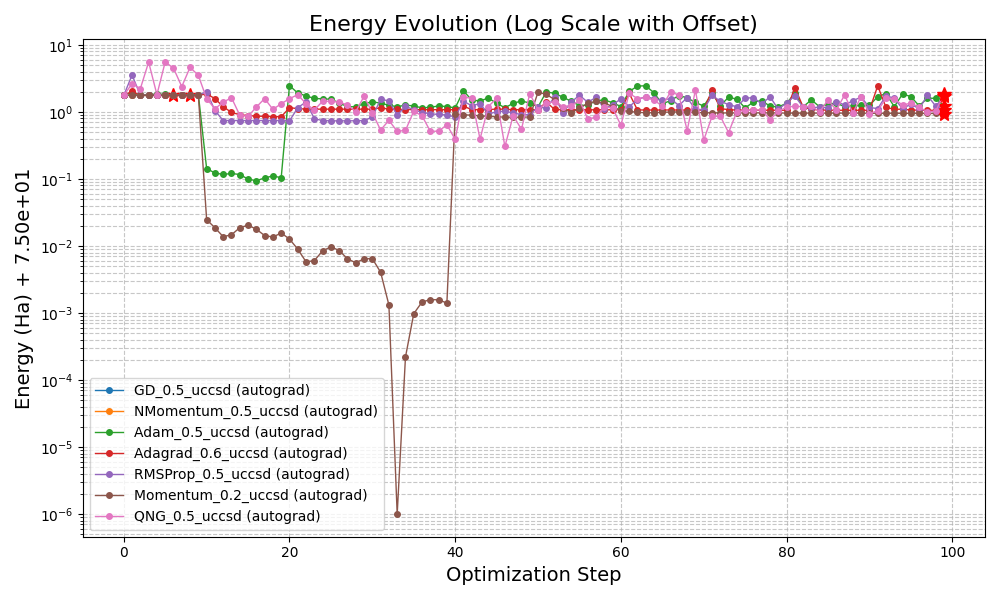
\includegraphics[width=\textwidth]{data/Optimizadores/final_results_H20/energy_evolution_log_offset.png}
    \caption{H2O simulation.}
    \label{fig:subimage3}
  \end{subfigure}
  \caption{Optimal \emph{step size} selection for each optimizer and molecule.}
  \label{fig:three_images}
\end{figure}

To delve deeper into the performance of the different optimizers, the following tables present the final energy, total optimization time, and the number of iterations required to converge for each molecule.

\begin{table}[H]
  \centering
  \caption{Final energy and optimization time for \(\mathrm{H_2}\), \(\mathrm{LiH}\), and \(\mathrm{H_2O}\) using various optimizers.}
  \begin{scriptsize}
  \begin{tabular}{lcccc}
  \toprule
  \textbf{Molecule} & \textbf{Optimizer} & \textbf{Final Energy (Ha)} & \textbf{Total Time (s)} & \textbf{Iterations} \\
  \midrule
  \multirow{7}{*}{\(\mathrm{H_2}\)} 
  & Adam (0.1)       & -1.07655292  & 173.30  & 10 \\
  & Adagrad (0.25)   & -1.13469066  & 10.19   & 1 \\
  & NMomentum (0.25) & -1.13730600  & 62.84   & 4 \\
  & Momentum (0.3)   & \(\mathbf{-1.13730605}\) & 100.43 & 6 \\
  & RMSProp (0.1)    & -1.13675411  & 33.14   & 2 \\
  & GD (0.3)         & \(\mathbf{-1.13730605}\) & 41.77  & 3 \\
  & QNG (0.1)        & -1.13469066  & 18.40   & 1 \\
  \midrule
  \multirow{7}{*}{\(\mathrm{LiH}\)} 
  & Adam (0.1)       & -7.87024707  & 13444.57 & 10 \\
  & Adagrad (0.2)    & -7.80548501  & 977.86   & 1 \\
  & NMomentum (0.05) & \(\mathbf{-7.87085783}\) & 13442.59 & 10 \\
  & Momentum (0.1)   & -7.75267240  & 13566.98 & 10 \\
  & RMSProp (0.15)   & -7.67650000  & 13671.22 & 10 \\
  & GD (0.02)        & -7.86422129  & 13449.49 & 10 \\
  & QNG (0.01)       & -7.85120449  & 13776.00 & 10 \\
  \midrule
  \multirow{7}{*}{\(\mathrm{H_2O}\)} 
  & Adam (0.5)       & -73.75990609 & 28454.49 & 10 \\
  & Adagrad (0.6)    & -73.93046296 & 28891.08 & 10 \\
  & NMomentum (0.5)  & -73.22152796 & 7497.83  & 1 \\
  & Momentum (0.2)   & \(\mathbf{-74.03997489}\) & 68420.47 & 10 \\
  & RMSProp (0.5)    & -73.28585876 & 65470.02 & 10 \\
  & GD (0.5)         & -73.22152796 & \(\mathbf{6486.79}\) & 1 \\
  & QNG (0.5)        & -73.13971041 & 70716.22 & 10 \\
  \bottomrule
  \end{tabular}
  \end{scriptsize}
\end{table}
  

In the evolution of the 3 iterations, we observed that the \textit{Momentum} optimizer was the one that offered the best performance in all the molecules. In the case of LiH, it is observed that it converges best until it reaches a geometric optimization, at which point it fails to converge. This is because the \emph{step size} is not yet fully optimized. Even so, we conclude that for the three simulations, the \textit{Momentum} optimizer is the one that offers the best performance.

An optimizer that also offers good performance is \textit{Adagrad}. Although it does not converge as effectively as \textit{Momentum}, it provides great speed in the simulations.

\newpage
\subsection{Step Size Selection}
To determine the most suitable \textit{step size} range, we started with the optimal value identified during optimizer selection. Subsequently, additional simulations were designed with values close to the initial optimum to refine this selection. 

This section presents the evolution of energy as a function of iterations, considering different \textit{step size} values for each molecule.

\begin{figure}[H]
  \centering
  % First image
  \begin{subfigure}{0.45\textwidth}
    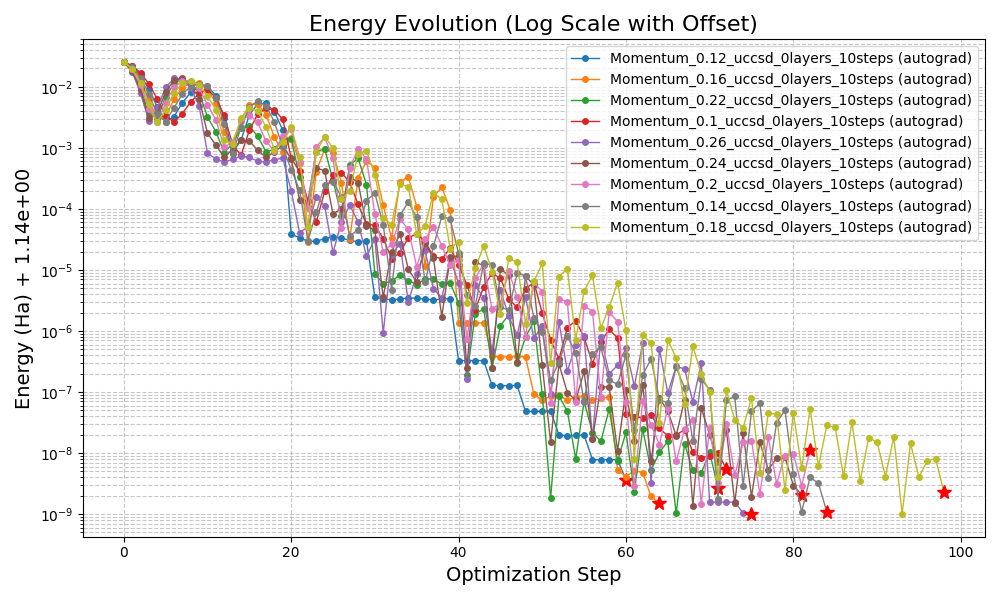
\includegraphics[width=\textwidth]{data/Stepsize/results_H2/energy_evolution_log_offset.png}
    \caption{H$_2$ simulation.}
    \label{fig:step_size_h2}
  \end{subfigure}
  % Second image
  \begin{subfigure}{0.45\textwidth}
    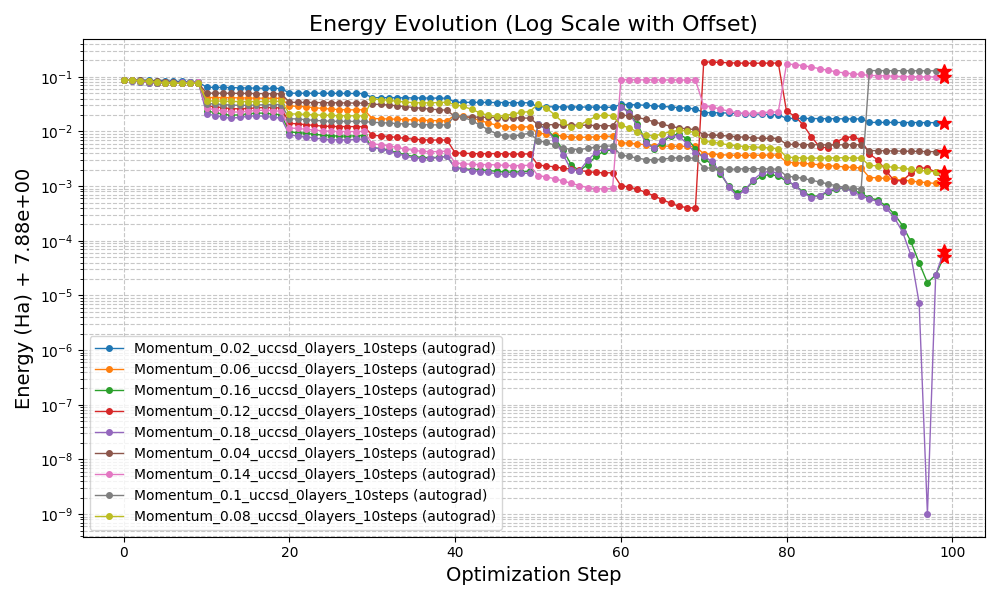
\includegraphics[width=\textwidth]{data/Stepsize/results_LiH/energy_evolution_log_offset.png}
    \caption{LiH simulation.}
    \label{fig:step_size_lih}
  \end{subfigure}
  % Third image
  \begin{subfigure}{0.45\textwidth}
    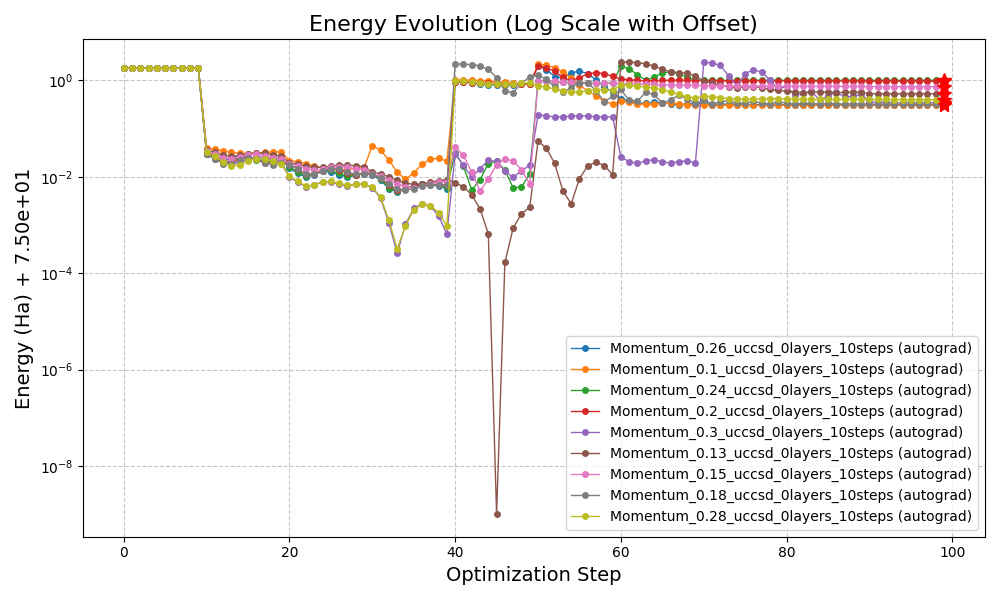
\includegraphics[width=\textwidth]{data/Stepsize/results_H2O/energy_evolution_log_offset.png}
    \caption{H$_2$O simulation.}
    \label{fig:step_size_h2o}
  \end{subfigure}
  \caption{Energy evolution as a function of \textit{step size} for different molecules.}
  \label{fig:step_size_results}
\end{figure}
Observing the graphs, we were able to see that for the molecules \(\mathrm{H_2}\) and \(\mathrm{LiH}\), the optimal \emph{step size} was clear, being 0.12 and 0.16 respectively. However, it was observed that for the molecule \(\mathrm{H_2O}\), the optimal \emph{step size} was not as clear, as there were several values that offered good performance.

For this reason, we created a table again to better observe the results. Note that in this case, each row corresponds to a \textit{step size}, keeping the same optimizer (  case, \textbf{Momentum}).

\begin{table}[H]
  \centering
  \caption{Final energy and optimization time for \(\mathrm{H_2}\), \(\mathrm{LiH}\), and \(\mathrm{H_2O}\) varying the \textit{step size} (optimizer: Momentum).}
  \begin{scriptsize}
  \begin{tabular}{lcccc}
  \toprule
  \textbf{Molecule} & \textbf{Step Size} & \textbf{Final Energy (Ha)} & \textbf{Total Time (s)} & \textbf{Iterations} \\
  \midrule
  \multirow{9}{*}{\(\mathrm{LiH}\)} 
  & 0.02 & -7.86678430 & \(\mathbf{13915.43}\) & 10 \\
  & 0.04 & -7.87699744 & 14001.06 & 10 \\
  & 0.06 & -7.88014045 & 13916.11 & 10 \\
  & 0.08 & -7.87944832 & 14144.26 & 10 \\
  & 0.10 & -7.75267240 & 14098.79 & 10 \\
  & 0.12 & -7.87992395 & 13937.66 & 10 \\
  & 0.14 & -7.78203292 & 14063.16 & 10 \\
  & 0.16 & \(\mathbf{-7.88118152}\) & 13931.81 & 10 \\
  & 0.18 & -7.88116774 & 13998.38 & 10 \\
  \midrule
  \multirow{9}{*}{\(\mathrm{H_2}\)} 
  & 0.10 & \(\mathbf{-1.13730605}\) & 113.23 & 10 \\
  & 0.12 & \(\mathbf{-1.13730605}\) & \(\mathbf{92.55}\) & 10 \\
  & 0.14 & \(\mathbf{-1.13730605}\) & 131.52 & 10 \\
  & 0.16 & \(\mathbf{-1.13730605}\) & 101.46 & 10 \\
  & 0.18 & \(\mathbf{-1.13730605}\) & 149.96 & 10 \\
  & 0.20 & -1.13730604 & 128.31 & 10 \\
  & 0.22 & \(\mathbf{-1.13730605}\) & 111.54 & 10 \\
  & 0.24 & \(\mathbf{-1.13730605}\) & 123.74 & 10 \\
  & 0.26 & \(\mathbf{-1.13730605}\) & 115.02 & 10 \\
  \midrule
  \multirow{9}{*}{\(\mathrm{H_2O}\)} 
  & 0.10 & \(\mathbf{-74.68985518}\) & 48577.15 & 10 \\
  & 0.13 & -74.46832273 & 74175.94 & 10 \\
  & 0.15 & -74.25355192 & 74211.21 & 10 \\
  & 0.18 & -74.67526296 & 75127.97 & 10 \\
  & 0.20 & -74.03997489 & 73130.72 & 10 \\
  & 0.24 & -73.99558215 & 56465.58 & 10 \\
  & 0.26 & -74.68963596 & \(\mathbf{44970.94}\) & 10 \\
  & 0.28 & -74.59437540 & 75555.08 & 10 \\
  & 0.30 & -74.65314486 & 73575.44 & 10 \\
  \bottomrule
  \end{tabular}
\end{scriptsize}
\end{table}

Finally, thanks to the table, we were able to see that, for \(\mathrm{H_2O}\), the \textit{step size} 0.10 was the one that gave the most optimal energy value, being slightly superior to 0.26.

Thus, we conclude that the optimal \textit{step size} values for the \textit{Momentum} optimizer are those found between 0.1 and 0.2, specifically, 0.12 for \(\mathrm{LiH}\), 0.12 for \(\mathrm{H_2}\), and 0.10 for \(\mathrm{H_2O}\).

\subsection{Number of Subiterations}

Finally, the last step that we performed to improve the performance of the simulation was in the number of subiterations that the optimization performs. By this, we refer to the iterations that are performed to optimize the parameters of each geometric position that we are optimizing the molecule. Since this is the process where most computational cost is incurred, it is a crucial step to improve the performance of the simulation.

To be able to configure in the most effective way the number of subiterations, we have generated a series of simulations with different numbers of subiterations, and we have observed the evolution of the energy. The configuration of the optimizers has been with the optimal values that we have obtained from the previous tests, with the Momentum optimizer and the step size values optimal for each molecule. Finally, the results have been compared with the values obtained from the following database: \href{https://cccbdb.nist.gov/}{NIST Computational Chemistry Comparison and Benchmark DataBase}.

Below are the graphs obtained from the different simulations:

\begin{figure}[H]
  \centering
  % First image
  \begin{subfigure}{0.45\textwidth}
    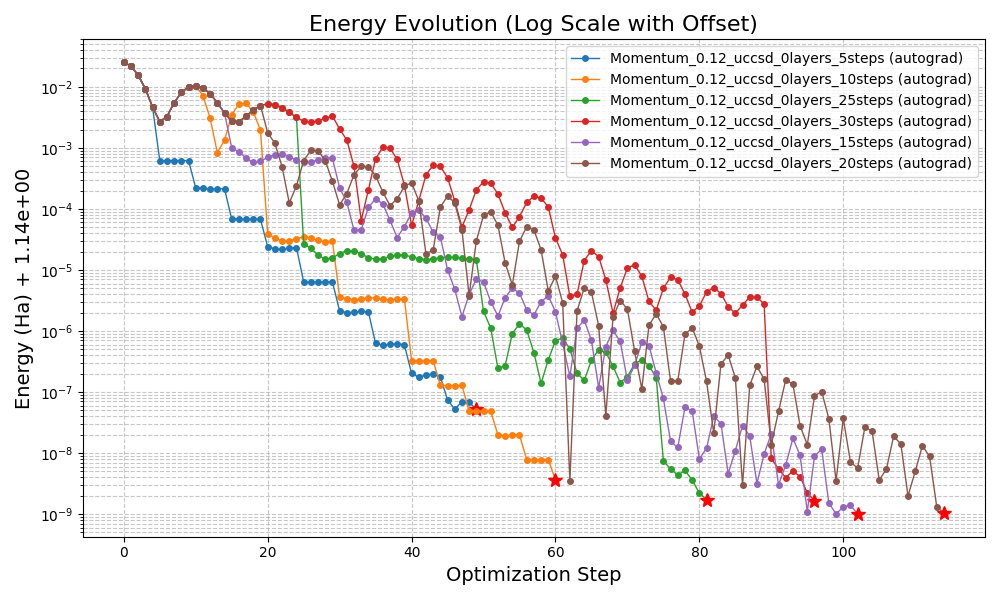
\includegraphics[width=\textwidth]{data/NumIterations/results_H2/energy_evolution_log_offset.png}
    \caption{H$_2$ simulation.}
    \label{fig:num_iterations_h2}
  \end{subfigure}
  % Second image
  \begin{subfigure}{0.45\textwidth}
    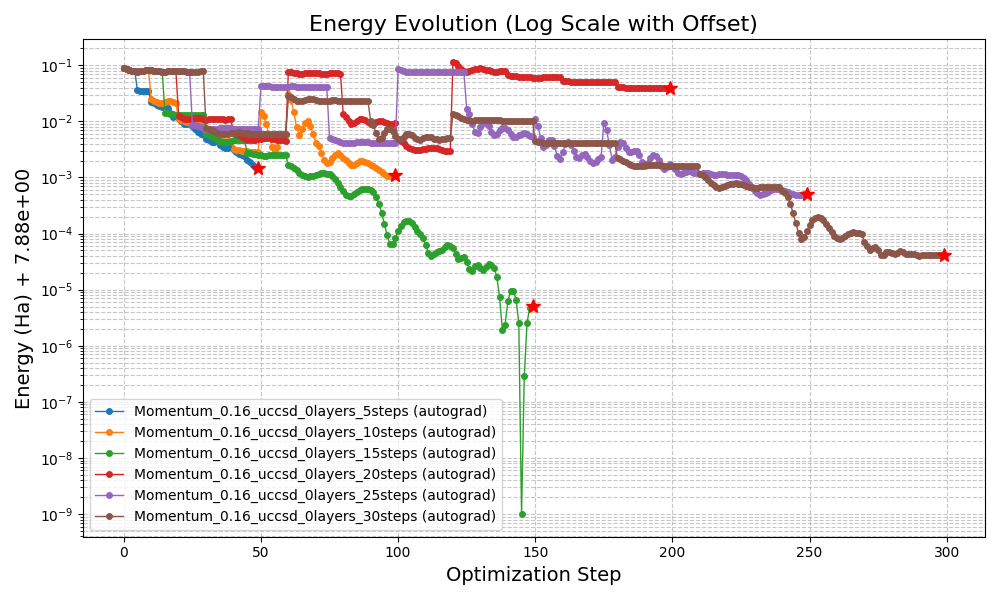
\includegraphics[width=\textwidth]{data/NumIterations/results_LiH/energy_evolution_log_offset.png}
    \caption{LiH simulation.}
    \label{fig:num_iterations_lih}
  \end{subfigure}
  % Third image
  \begin{subfigure}{0.45\textwidth}
    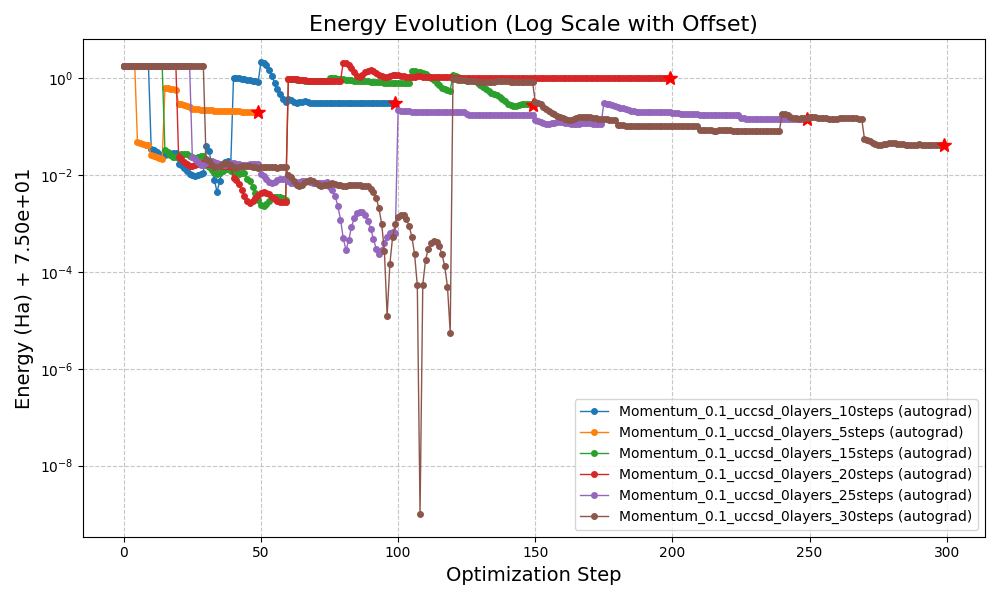
\includegraphics[width=\textwidth]{data/NumIterations/results_H2O/energy_evolution_log_offset.png}
    \caption{H$_2$O simulation.}
    \label{fig:num_iterations_h2o}
  \end{subfigure}
  \caption{Energy evolution as a function of \textit{number of iterations} for different molecules.}
  \label{fig:num_iterations_results}
\end{figure}

\subsubsection{Initial Results}

As in previous sections, to clarify the results, we have generated tables of the results that serve as tools for analyzing the outcomes in greater depth.

\begin{table}[H]
  \centering
  \caption{Final energy and optimization time for \(\mathrm{H_2}\), \(\mathrm{LiH}\), and \(\mathrm{H_2O}\) using Momentum optimizer with varying steps.}
  \begin{scriptsize}
  \begin{tabular}{lcccc}
  \toprule
  \textbf{Molecule} & \textbf{Steps} & \textbf{Final Energy (Ha)} & \textbf{Total Time (s)} & \textbf{Difference from FCI (Ha)} \\
  \midrule
  \multirow{6}{*}{\(\mathrm{H_2}\)} 
  & 5  & \(\mathbf{-1.13730605}\) & 101.86 & 0.00000005 \\
  & 10 & \(\mathbf{-1.13730605}\) & \(\mathbf{99.08}\) & 0.00000005 \\
  & 15 & \(\mathbf{-1.13730605}\) & 163.25 & 0.00000005 \\
  & 20 & \(\mathbf{-1.13730605}\) & 175.06 & 0.00000005 \\
  & 25 & \(\mathbf{-1.13730605}\) & 124.58 & 0.00000005 \\
  & 30 & \(\mathbf{-1.13730605}\) & 147.59 & 0.00000005 \\
  \midrule
  \multirow{6}{*}{\(\mathrm{LiH}\)} 
  & 5  & \(-7.88079149\) & \(\mathbf{8328.30}\) & 0.00174651 \\
  & 10 & \(-7.88118152\) & 13365.38 & \(\mathbf{0.00135648}\) \\
  & 15 & \(-7.88226478\) & 18384.78 & 0.00027322 \\
  & 20 & \(-7.84260017\) & 23309.87 & 0.03993783 \\
  & 25 & \(-7.88176386\) & 28433.90 & 0.00077414 \\
  & 30 & \(\mathbf{-7.88222895}\) & 33421.15 & \(\mathbf{0.00030905}\) \\
  \midrule
  \multirow{6}{*}{\(\mathrm{H_2O}\)} 
  & 5  & \(-74.79245495\) & \(\mathbf{50836.87}\) & \(0.22251505\) \\
  & 10 & \(-74.68985518\) & 45559.48 & \(0.32511482\) \\
  & 15 & \(-74.70554258\) & 77448.07 & \(0.30942742\) \\
  & 20 & \(-74.00851054\) & 113172.24 & \(1.00645946\) \\
  & 25 & \(-74.84425344\) & 136497.21 & \(0.17071656\) \\
  & 30 & \(\mathbf{-74.94705746}\) & 157949.56 & \(\mathbf{0.06791254}\) \\
  \bottomrule
  \end{tabular}
  \end{scriptsize}
\end{table}

  
We clearly observe that for the molecule \(\mathrm{H_2}\), the number of subiterations does not affect the final result. In this case, as it is such a basic molecule with few parameters, the simulation converges relatively easily for all configurations. Thus, we observe that the best option, due to its speed and accuracy, and yielding the best performance, is the configuration with 10 subiterations per geometric position, with an execution time of 99.08 seconds, being 2.72\% faster than the configuration with 5 subiterations.

In the case of \(\mathrm{LiH}\), the energy \(-7.88222895\,\mathrm{Ha}\) achieved in 30 steps shows the best accuracy compared to the reference value. However, as we are interested in a balance between performance and accuracy, by observing the execution times and results, we find that the optimal performances are achieved with a number of subiterations between 5 and 10 per geometric optimization cycle. Considering that the accuracy with 10 subiterations is 22.33\% higher but with a 37.68\% increase in computation time, we conclude that the process with highest efficiency is that with 5 subiterations.

For the molecule \(\mathrm{H_2O}\), we find the same result as for the molecule \(\mathrm{LiH}\), where the highest accuracy is obtained with 30 subiterations, but the best performance is achieved with 5 to 10 subiterations per cycle. Making the same comparison as before, we find that with 10.38\% less computation, we obtain 31.55\% less accuracy, so the optimal performance is achieved with 5 subiterations.

The results show that highest efficiency is found between 5 and 10 subiterations per geometric optimization cycle, achieving a balance between accuracy and computation time. This leads us to conclude that the best option is 10 subiterations for the molecule \(\mathrm{H_2}\), and 5 subiterations for the molecules \(\mathrm{LiH}\) and \(\mathrm{H_2O}\). For this reason, we have decided to analyze how these molecules evolve with this number of subiterations. The results obtained are presented below.

\subsubsection{Final phase}
To find a more precise value for the optimal number of subiterations, we conducted the same simulations as in the previous sections, but varying the number of subiterations in our simulations, setting them to values from 2 to 10. This allowed us to observe more clearly how the hybrid optimization technique implemented in our project affects the results.

\begin{figure}[H]
  \centering
  % First image
  \begin{subfigure}{0.45\textwidth}
    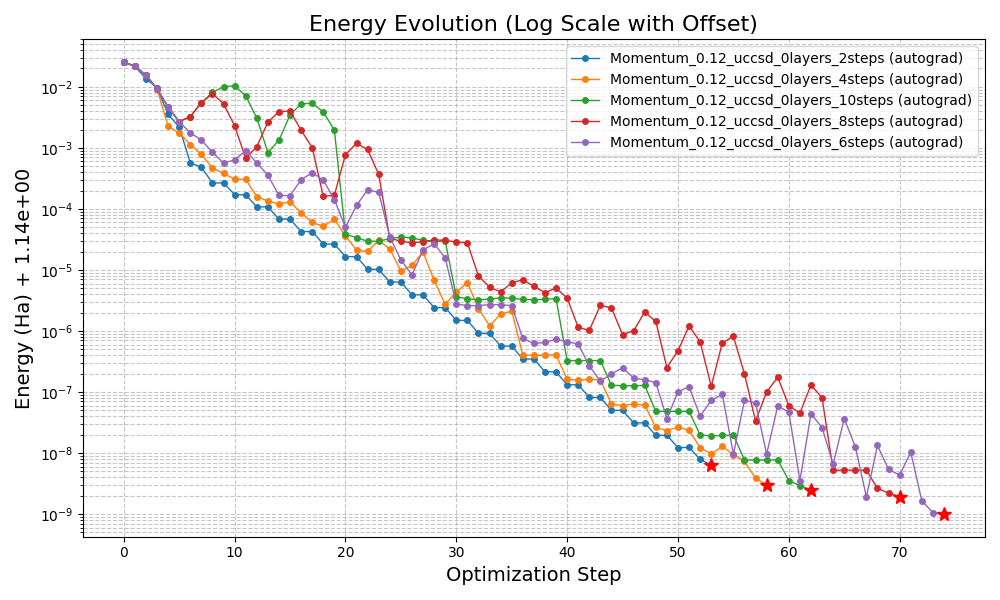
\includegraphics[width=\textwidth]{data/NumIterations/final_results_H2/energy_evolution_log_offset.png}
    \caption{H$_2$ simulation.}
    \label{fig:num_iterations_final_h2}
  \end{subfigure}
  % Second image
  \begin{subfigure}{0.45\textwidth}
    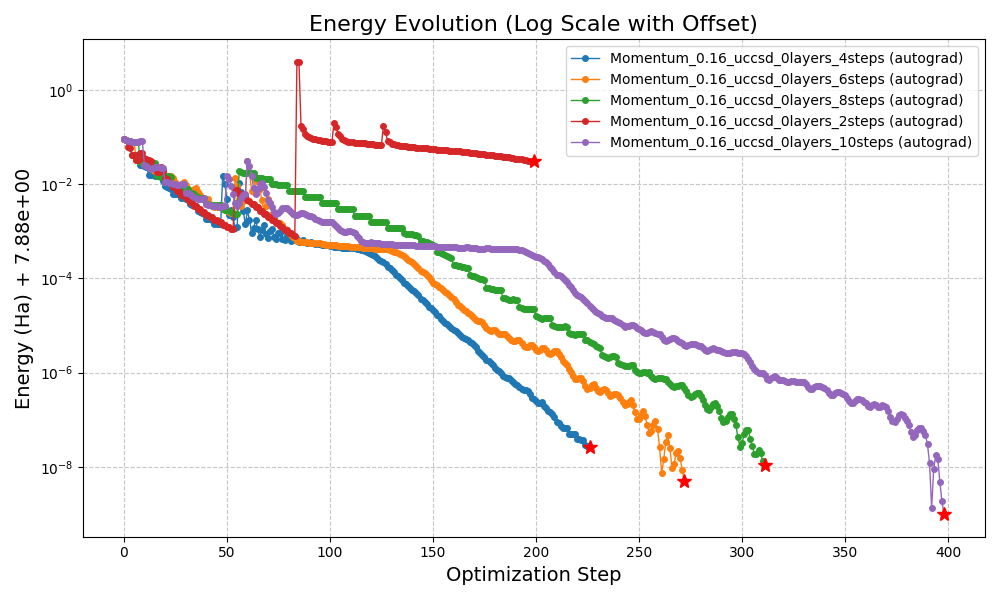
\includegraphics[width=\textwidth]{data/NumIterations/final_results_LiH/energy_evolution_log_offset.png}
    \caption{LiH simulation.}
    \label{fig:num_iterations_final_lih}
  \end{subfigure}
  % Third image
  \begin{subfigure}{0.45\textwidth}
    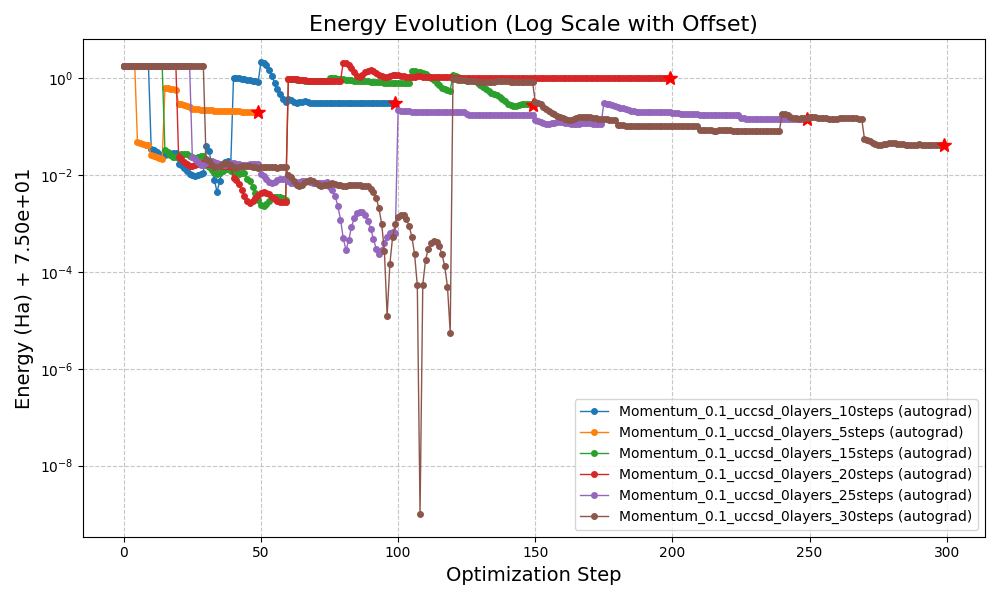
\includegraphics[width=\textwidth]{data/NumIterations/results_H2O/energy_evolution_log_offset.png}
    \caption{H$_2$O simulation.}
    \label{fig:num_iterations_final_h2o}
  \end{subfigure}
  \caption{Energy evolution as a function of \textit{number of iterations} for different molecules.}
  \label{fig:num_iterations_final_results}
\end{figure}
In the graphs obtained from this second simulation, the effect of hybrid optimization on convergence is clearly observed. The fewer the number of subiterations, the faster the convergence. However, this has a negative effect, as the optimization becomes more unstable and imprecise. We observe that in the molecule \(\mathrm{H_2}\), convergence is faster with 2 subiterations. In the case of \(\mathrm{LiH}\), the most effective simulation is with 4 subiterations. Additionally, it is observed that reducing to 2 subiterations causes the simulation to fail to converge due to the instability of the optimization. The data from both simulations are presented below.

\begin{table}[H]
  \centering
  \caption{Final energy and optimization time for \(\mathrm{H_2}\) and \(\mathrm{LiH}\).}
  \begin{scriptsize}
  \begin{tabular}{lcccc}
  \toprule
  \textbf{Molecule} & \textbf{Steps} & \textbf{Final Energy (Ha)} & \textbf{Total Time (s)} & \textbf{Difference from FCI (Ha)} \\
  \midrule
  \multirow{5}{*}{\(\mathrm{H_2}\)} 
    & 2  & \(-1.13730605\) & \textbf{95.57}  & \(0.00000005\) \\
    & 4  & \(-1.13730605\) & 96.65   & \(0.00000005\) \\
    & 6  & \(-1.13730605\) & 122.50  & \(0.00000005\) \\
    & 8  & \(-1.13730605\) & 111.27  & \(0.00000005\) \\
    & 10 & \(-1.13730605\) & 98.74   & \(0.00000005\) \\
  \midrule
  \multirow{5}{*}{\(\mathrm{LiH}\)} 
    & 2  & \(-7.85253665\) & 51461.91 & \(0.03000135\) \\
    & 4  & \(\mathbf{-7.88275270}\) & \(\mathbf{40118.76}\) & \(\mathbf{0.00021470}\) \\
    & 6  & \(-7.88275272\) & 40896.30 & \(0.00021472\) \\
    & 8  & \(-7.88275272\) & 43240.40 & \(0.00021472\) \\
    & 10 & \(-7.88275272\) & 43240.40 & \(0.00021472\) \\
  \bottomrule
  \end{tabular}
  \end{scriptsize}
\end{table}

\section{Limitations}
During the tests conducted, we identified various limitations that may have affected the results. The most significant limitation has been the lack of implementation of quantum error simulations. In all simulations, the negative effects of errors that can occur in real quantum computers have not been considered. For this reason, we cannot assert that these same results would be useful for a similar implementation on a real quantum computer.

Similarly, we did not have access to a quantum computer, which would have been extremely helpful in validating the proper functionality of our project. Even so, we have been able to verify that our project performs optimally and that the implementation of hybrid optimization is effective in improving the performance of the simulations.

Another limiting aspect has been the computational capacity of our computer. Since we do not have access to a quantum computer, simulations with a high number of molecules have been very costly in terms of computational time.